

\cs{@gbt @mw}
\subsection{Overview of ManyNames}
\label{sect:mn_overview}

brief summary of lrec paper, shortcoming, what we added

\subsection{Verification of Annotations}
\label{sect:mn_verification}

\mw{Below can be shortened no doubt; but could also be moved to appendix. Plz. let me know what you consider the most appropriate (I'm an ACL noobie).}

Although the initial data gathering phase involved some very basic quality control (detecting repeated names, empty text fields, typos), we had no rigorous way of ascertaining that our participants were providing adequate names for the intended object.
Given our high number of annotators in phase 1 we decided to simply discard names that were entered by only one annotator.
Moreover, for images where all 36 annotators entered the same name we decided to take this name to be adequate. 
That still leaves 19427 images, with on average 4 names each, to be properly verified, which we did as follows.

We conducted a second round of annotation where we asked people whether each name for a given image was adequate and, if not, what type of inadequacy it was.
Moreover, we asked them to indicate which names were likely intended for the same real-world object.
The task interface is shown in figure~\ref{fig:verification-interface} in the appendix.
Adequacy was rated on a 3-point scale from ``perfectly adequate'' to ``there may be a (slight) inadequacy'' to ``totally inadequate'', represented by appropriate emotes.
We provided (and clarified by means of explanation and visual examples) the following definition: \textit{a name is ``adequate'' if there is an object in the image, whose visible parts are tightly circumscribed by the red bounding box, that one could reasonably call by that name}.
When the participant selected slightly or totally inadequate, four additional icons would appear to indicate the type of inadequacy: ``linguistic mistake'', ``named object not tightly in bounding box'', ``named object mistaken for something it's not'', and ``something else''.
We provided detailed instructions and examples at the top, as well as informative hover texts on all the buttons.

Because the quality of the data we gather in this phase will be essential for gaining insight into the ManyNames dataset, as well as for evaluating computational models (section~\ref{sec:experiments}), we conducted rigorous quality control.
Every task included around 15\% automatically generated quality control items of various kinds (names for objects in a different image, names for other objects in the same image, WordNet synonyms of given names, inserted typos, and more).
When trying to submit their results, participants would get a warning if their accuracy on these items was below 90\%, and the advice to stop doing these tasks if it was below 80\%, with the option to double-check their responses.
They would get a bonus of \$0.15 if all control items were answered correctly (happened about half the time).
After every round we blocked annotators with low ($<$90\%) average accuracy, removed their results from the dataset and republished the relevant tasks to ensure consistent coverage of our data.

We implemented this verification task on Amazon Mechanical Turk (\url{https://mturk.com}). 
Basic numbers and results are reported in Table~\ref{tab:verification-numbers}.
\begin{table}[t]
	\centering
	\small
	\begin{tabular}{|ll|ll|}
		\hline
		\multicolumn{2}{|c|}{\textbf{Task setup:}} & \multicolumn{2}{c|}{\textbf{Results:}} \\ \hline
		Images: & 19427 &
			Annotators: & 255 \\
		Img-name pairs: & 69356 &
			Annotators/task: & $\geq$ 3 \\
		Tasks: & 3052 &
			Adeq. mean: & \hspace{-3em}.80 (std .093)\\
		Images/task: & 6-7 &			
			Agreement (adeq.) & 88\% \\ 
		Names/task: & 20-30 &
			Agr. (inadeq. type): & 86\% \\
		\multicolumn{2}{|l|}{Task reward: \ \$.50 (+.15)} & 
			Agr. (same-obj): & 94\% \\
		\hline
	\end{tabular}
	\caption{Verification task overview.}
	\label{tab:verification-numbers}
\end{table}
Average name adequacy, encoded on a scale $[0,1]$, is 0.80 with small standard deviation (0.093). 
Inter-annotator agreement is high also by other measures: the proportion of annotators agreeing on ``adequate'' is 88\%, agreeing on inadequacy type is 86\%, and agreeing on whether two names were intended for the same object is 94\%.
This level is agreement is high given the complexity of the task (e.g., pictures sometimes unclear), especially bearing in mind that we essentially asked our participants to do some kind of mind-reading (i.e., which object could someone who entered an inadequate name plausibly have had in mind?).
Figure~\ref{fig:verification-piechart} shows the proportion of `adequate' judgments and the types of inadequacies our annotators reported.
\begin{figure}[t]
	\centering
	\hspace*{.2\columnwidth}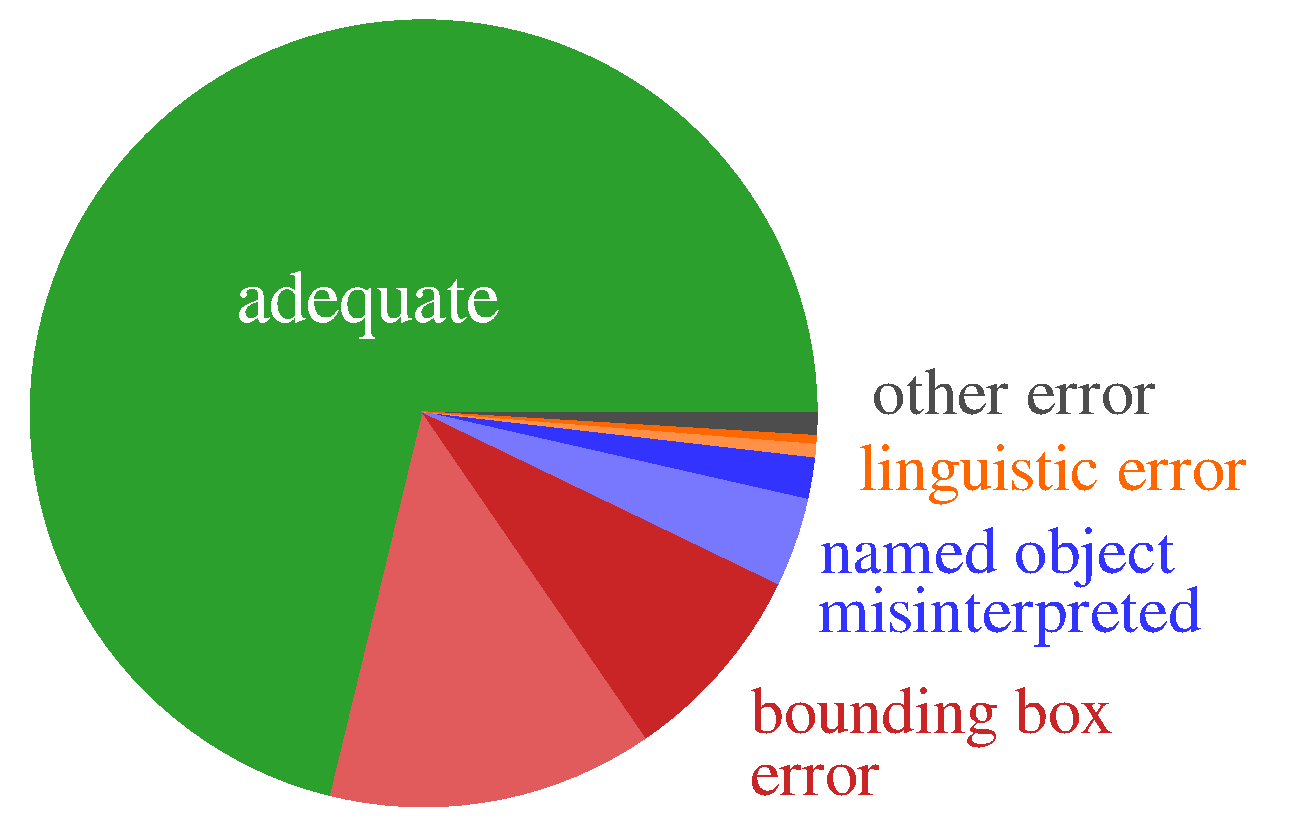
\includegraphics[width=.7\columnwidth]{images/verification_piechart.pdf}
	\caption{Verification results (counting individual annotations). Lighter shade within a hue indicates slight/possible error of that type; darker shade severe error.}
	\label{fig:verification-piechart}
\end{figure}
\mw{Possibly a pie-chart counting actual names and their aggregated (+thresholded) scores would be more informative than the current pie-chart, which counts original (i.e., non-aggregated) verification annotations.}

We aggregate our name adequacy judgments (representing adequate as 1, slightly inadequate as 0.5 and totally inadequate as 0) by taking the mean, and inadequacy type judgments by taking the majority (also counting ``none'' if there was no inadequacy).
As for the judgments of whether two names were intended for the same object, we use two different types of aggregations, for different purposes.
For evaluating computational object naming models, we want to know primarily whether a name generated by a model could have been intended to name the same object as the entry-level name (i.e., the most frequent name).
This we compute by a simple majority rule: true if name1 and name2 were judged to be for the same object by a majority of annotators, and false otherwise.
However, we are also interested in more general statistics, e.g., the mean number of names per object, and the relative frequencies of names for a given object.
For this, we need to compute clusters of names (the pairwise majority rule does not result in a proper clustering): as distance between names we use the proportion of annotators saying they do not name the same object, and we perform agglomerative, complete-linkage clustering with a threshold of .5 (i.e., all pairs of names in a cluster must name the same object according to a majority of annotators).
A possible disadvantage of this (hard) clustering method is that every name can only be in one cluster, i.e., name only one object.
It entails for instance that \emph{food} cannot be clustered both with \emph{pizza} and with the \emph{cheese} on top, even though both are definitely instances of food.
But this is not as problematic as it may seem, because we do not care primarily about such taxonomic relationships (which could be gotten from, e.g., WordNet) -- rather, we care about (and asked our annotators) which single object a person who entered \emph{food} was likely intending to name: presumably the pizza as a whole rather than the cheese on top.
Moreover, although (hard) clustering may occasionally lead us to \emph{under}estimate the number of names for an object, the alternative, \emph{soft} clustering (where each name could potentially be in multiple clusters) would risk \emph{over}estimating the number of names per object, as well as the number of named objects in an image, both of which would be more harmful to our aims.

% We relied on 255 mostly recurring workers, who did a total of 9491 published tasks.
% Each task would present the worker with 6 or 7 images, for a total of between 20 and 30 names.
% We offered a reward of \$0.50 with an additional bonus of \$0.15 if all control items were % answered correctly as extra incentive (which happened about half the time).
% Our approach was valued by the workers for the interesting task, natural interface and good reward.


\subsection{Analysis}
\label{sect:mn_analysis}

\cs{+ @sz?}\\
\cs{Here goes what has not been discussed in LREC paper, because it focusses on entry-level names. }
\cs{Results aimed to show that we need \underline{multiple} annotations per object \underline{instance} to get the entry-level name}

\paragraph{Definition of ``Entry-level Name''} \sz{has this been mentioned before?}
\mw{I'd definitely put this in the introduction, and leave only a reminder here.}
In the following, we consider a name annotated for an object as an entry-level name if it corresponds to the most frequent name given a set of name annotations for an object.
\mw{We could also consider defining entry-level name as `the most frequent adequate name'? Or perhaps as `the most frequent name \emph{if it is adequate}, none otherwise'? Depending on what makes the narrative easier.}

\mw{Also make sure to define the notion of `entry-level object', or `canonical object' perhaps? i.e., the object/cluster of the entry-level name.}

\paragraph{Entry-level Names in ManyNames:} As shown in Table \ref{tab:stat-entry-level}, ManyNames provides a large vocabulary of names (7970) for 25K objects. Note that this vocabulary is much larger than what state-of-the-art object detectors are typically trained on. The vocabulary of entry-level names is drastically smaller and contains only 442 types. This small set, however, covers at least 50\% of the objects in VisualGenome, i.e. almost 2M objects in VisualGenome are mentioned in a region descriptions with one of these 442 entry-level names.

\begin{table}[t]
	\centering
	\small
	\begin{tabular}{p{5cm}l}
		\toprule		
\# objects in MN & 25,315\\
total vocab  &  7,970\\
entry-level vocab & 442\\
\# objects with entry-level name in VG & $\sim$ 2M (50\%)\\
\midrule
av. agreement all names & 34.9\%\\
av. agreement entry-level names & 75.2\%\\
av. agreement entry-level cluster & 42.3\%\\
\midrule
av. adequacy all names & 0.81\\
av. adequacy entry-level names & 0.97 \\
av. adequacy entry-level cluster & 0.94 \\
\bottomrule	
	\end{tabular}
	\caption{Basic statistics for entry-level names in MN}
	\label{tab:stat-entry-level}
\end{table}

\paragraph{Entry-level Names are Instance-Dependent:} In a traditional, taxonomic view of object naming, entry-level names can be determined solely based on the object's class, meaning that all instances of a class have the same entry-level name. The MN data provides evidence that this is not the case, even though we do not have access to ground-truth class annotations in \vg (we only have names). Instead, we observe that there are many pairs of entry-level names that do not have a fixed preference ordering across instances, as illustrated in Figure \ref{fig:duck} where the rather non-prototypical instance of a \textit{duck} is named \textit{bird} by most annotators. We find that there are 879 pairs of entry-level names that show a different preference ordering depending on the instance (e.g. \textit{boy-player}, \textit{sandwich-food}, \textit{building-church}, ...).


\sz{does this solve this? Statistics wrt entry-level of object class != entry-level of its instances to (i.e.,\ entry-levels cannot be derived on class-level)} \gbt{But, what's an object class in our data? We can't really use collection synsets, can we? Those are not really object classes?} \gbt{UPDATE: We change focus from class to ``entry-level names are instance-specific''. Matthijs is on it.}


\sz{somewhere we should mention these tendencies on adequacy and agreement for (non-)entry-level names shown in Table \ref{tab:stat-entry-level}}


\paragraph{Identifying entry-level names requires many annotators}
ManyNames was collected in four rounds of 9 annotators each.
On average, the most frequent names differed between rounds for 20\% of objects (std.dev. 2.4\%p), suggesting that entry-level names cannot be reliably identified from too few annotators.
Figure~\ref{fig:entry-level-name-stability} shows this in a more general way.
\mw{@gbt: I first did it the way you suggested, i.e., by sampling, but I found the resulting plot (not shown now) too hard to interpret, even a bit misleading. I've kept this text + plot in the TeX source further below, commented out, in case you want to have a look. But I think the following is better:}
\begin{figure}[t]
	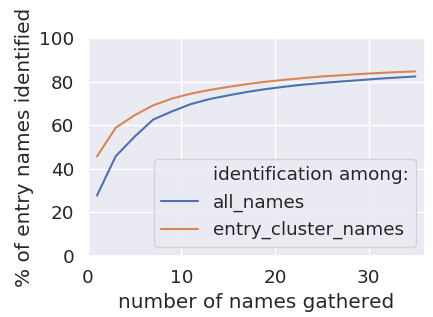
\includegraphics[width=\columnwidth]{images/stability_analytic.png}
	\caption{Proportion of objects (vertical) for which the entry-level name can be confidently (95\%) identified after gathering N names (horizontal). \mw{increase plot font size}}
	\label{fig:entry-level-name-stability}
\end{figure}
For each object we computed, on the basis of the distribution of names in ManyNames for that object, how many names should have been gathered for the majority name among them to be the entry-level name (as defined on the basis of 36 names) with 95\% probability (a reasonable confidence requirement).
The blue line shows that, even after gathering 10 names, the majority name is this likely to be the entry-level name for only 68\% of objects (put differently: for the remaining 32\% of objects, there's a greater than 5\% chance of getting a different majority name).
Gathering 20 names increases this to 78\%.
The red line shows the same tendency but by taking only names from the entry-level cluster into account (as identified by our Verification results):
by discarding names for other objects, the entry-level name for the intended object can be confidently identified slightly more quickly (but not by much, since names for the wrong object tend to be a minority anyway).
Both lines level level out well below 100\%, reflecting that for 15\%-20\% \cs{Can you compute that individually for each domain?} of objects even gathering 36 names is not enough for the entry-level name to come out as majority with 95\% probability: differences in frequencies between the contenders are simply too small.
\mw{@cs, @sz, @gbt: A closely related (but different) question this immediately brings to mind (of a critical reviewer?) is: how sure are we, for a given object, given the particular names we gathered, that the most frequent name in our sample (what we \emph{call} the entry-level name) is indeed the most frequent name in the population (what actually \emph{is} the entry-level name, right?)? Should we address this question earlier? I think the stats will look very similar (though they're not the same): that for 15-20\% of objects we really aren't sure.}

%%%%%% BY SAMPLING, FOR GEMMA:
% For each object that has an adequate entry-level name (adequacy $<.5$ according to our Verification results), we randomly sampled (including duplicates) a list of 36 names using the proportions in ManyNames as sampling probabilities, and computed the lowest number of collected names (i.e., the lowest index in the list) after which the entry-level name would reliably remain the most frequent one.
% We did this 30 times for each object.
% The blue line in the figure shows that, after collecting 10 names, the entry-level name is reliably identified for on average around 85\% of objects; collecting 20 names increases this to 90\%.\footnote{
%	But even when gathering 36 names, for around 6\% of objects this can still result in a different entry-level name. This reflects the existence of objects with no clear entry-level name, e.g., where two (almost) equally frequent names are both candidates.
%	\mw{Can we quantify this?}
%}
%The red line shows the same tendency but by taking only names from the entry-level cluster into account (as identified by our Verification results):
%by discarding names for other objects, the entry-level name for the intended object can be identified slightly more quickly (but not by much, since names for the wrong object tend to be a minority anyway).
%\begin{figure}[t]
%	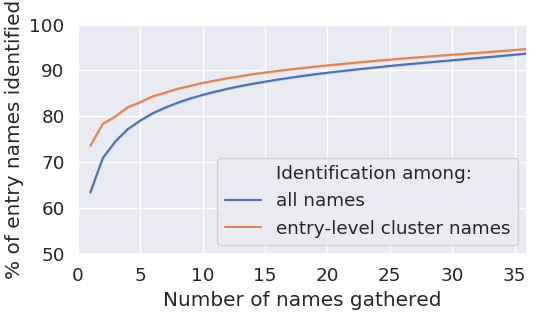
\includegraphics[width=\columnwidth]{images/stability-all-05-05-spellchecked.png}
%	\caption{}
%	\label{fig:entry-level-name-stability}
%\end{figure}

\paragraph{Of Verification Annotations}

\cs{@gbt @mw}



\begin{itemize}
	\item ...
	\item ...
	\item For the instances where VG!=topMN: Percentage of instances where the VG name is among the responses of an \textit{alternative object} (as given by clustering).
	\item Comparison of VG and MN, demonstrating that MN is a more reliable source for entry-level names. 
\end{itemize}


%%% Local Variables:
%%% mode: latex
%%% TeX-master: "acl2020_main"
%%% End:
